\section{Introduction}
\label{sec:intro}

% Intro to Adaptive Analysis

The computational complexity of most problems is studied in the worst
case over instances of fixed size $n$, for $n$ asymptotically tending
to infinity. This approach was refined for NP-difficult problems under
the term ``parameterized
complexity''~\cite{2006-BOOK-ParameterizedComplexityTheory-FlumGrohe},
for polynomial problems under the term ``Adaptive
Algorithms''~\cite{1992-ACMCS-ASurveyOfAdaptiveSortingAlgorithms-EstivillCastroWood,1992-ACJ-AnOverviewOfAdaptiveSorting-MoffatPetersson},
and more simply for data encodings under the term of ``Data
Compression''~\cite{2013-TCS-OnCompressingPermutationsAndAdaptiveSorting-BarbayNavarro},
for a wide range of problems and data types.
Such a variety of results has motivated various tentative to classify
them, in the context of NP-hard problems with a theory of Fixed
Parameter
Tractability~\cite{2006-BOOK-ParameterizedComplexityTheory-FlumGrohe},
and in the context of sorting in the comparison model with a theory of
reduction between
parameters~\cite{1995-DAM-AFrameworkForAdaptiveSorting-PeterssonMoffat}.

% Examples of Results and Classification in Adaptive Analysis

In the context of ``Adaptive Analysis of Algorithms'', we introduce
two other perspectives from which to classify algorithms and data
structures: those taking advantage of the \emph{input order} (e.g.,
disorder measures for
\textsc{Sorting}~\cite{1992-ACJ-AnOverviewOfAdaptiveSorting-MoffatPetersson,1992-ACMCS-ASurveyOfAdaptiveSortingAlgorithms-EstivillCastroWood},
\textsc{Convex Hull}
algorithms~\cite{2002-SWAT-AdaptiveAlgorithmsForConstructingConvexHullsAndTriangulationsOfPolygonalChains-LevcopoulosLingasMitchell})
and those taking advantage of the \emph{input structure} (e.g., output
sensitive
algorithms~\cite{1986-JCom-TheUltimatePlanarConvexHullAlgorithm-KirkpatrickSeidel},
input order oblivious instance
optimality~\cite{2009-FOCS-InstanceOptimalGeometricAlgorithms-AfshaniBarbayChan}).

By \emph{input order} we mean algorithms taking advantage of the order
of the input, for example, taking advantage of the order of the values
in a sequence of numbers or of the order in which the points are given
in a polygonal chain.

% input order sorting
Concerning the \textsc{Sorting} problem, as early as 1973,
Knuth~\cite{1973-BOOK-TheArtOfComputerProgrammingVol3-Knuth} described
a variant of the algorithm {\tt{MergeSort}} that sorts an array
$\mathcal{A}$ using a prepossessing step taking linear time to detect
maximal sorted subblocks, called \emph{runs}, in $\mathcal{A}$.
Takaoka~\cite{2009-Chapter-PartialSolutionAndEntropy-Takaoka}
described a new sorting algorithm that optimally takes advantage of
the distribution of the sizes of the runs in the array $\mathcal{A}$,
which yields a time complexity within
$O(n(1+\mathcal{H}(r_1, \dots, r_{\rho}))) \subseteq
O(n(1{+}\log{\rho})) \subseteq O(n\log{n})$, where $\rho$ is the
number of runs in $\mathcal{A}$ and $r_1, \dots, r_{\rho}$ are the
sizes of the $\rho$ \emph{runs} (such that $\sum_{i=1}^\rho {r_i}=n$),
respectively. Takaoka measures the ``difficulty'' of the instance in
terms of the ``input order'' by the entropy function
$\mathcal{H}(r_1, \dots, r_\sigma) =
\sum_{i=1}^\sigma{\frac{r_i}{n}}\log{\frac{n}{r_i}}$. These results
take advantage of the order of the values in the input i.e., the input
order.

% input order convex hull
Considering the computation of the {\sc{Convex Hull}} in the plane,
Levcopoulos et
al.~\cite{2002-SWAT-AdaptiveAlgorithmsForConstructingConvexHullsAndTriangulationsOfPolygonalChains-LevcopoulosLingasMitchell}
described a divide-and-conquer algorithm for computing the {\sc{Convex
    Hull}} of a polygonal chain. They measured the complexity of this
algorithm in terms of the minimum number of simple subchains $\kappa$
into which the chain can be cut.  They showed that the time complexity
of this algorithm is within
$O(n(1{+}\log{\kappa})) \subseteq O(n\log{n})$. This result takes
advantage of the order in which the points are given i.e., the input
order.

By ``input structure'' we mean algorithms taking advantage of the structure of the instance, for example, taking advantage of the frequencies of the values in a multiset or of the relative positions of the points in a set.

Concerning the {\sc{Sorting}} problem, Munro and
Spira~\cite{1976-JComp-SortingAndSearchingInMultisets-MunroSpira}
considered the task of {\sc{Sorting}} a multiset
$S=\{x_1, \dots, x_n\}$ of $n$ real numbers with $\sigma$ distinct
values, of multiplicities $m_1, \dots, m_\sigma$ (such that
$\sum_{i=1}^\sigma {m_i}=n$), respectively. They showed that adding
counters to various classical algorithms
\begin{INUTILE}
  (among which the divide-and-conquer based algorithm
  {\tt{MergeSort}})
\end{INUTILE}
yields a time complexity within
$O(n(1+\mathcal{H}(m_1, \dots, m_\sigma))) \subseteq
O(n(1{+}\log{\sigma})) \subseteq O(n\log{n})$ for {\sc{Sorting}} a
multiset. This result takes advantage of
the frequencies of the values i.e., the structure of the instance.

Considering the problem of computing the {\sc{Convex Hull}}, Kirkpatrick and Seidel~\cite{1986-JCom-TheUltimatePlanarConvexHullAlgorithm-KirkpatrickSeidel} described an algorithm to compute the {\sc{Convex Hull}} of a set of $n$ planar points in time within $O(n(1+\log h))\subseteq O(n\log n)$, where $h$ is the number of vertices in the {\sc{Convex Hull}}.
\begin{INUTILE}
  The algorithm relies on a variation of the divide-and-conquer
  paradigm, which they call the ``Marriage-Before-Conquest''
  principle.
\end{INUTILE}
Afshani et al.~\cite{2009-FOCS-InstanceOptimalGeometricAlgorithms-AfshaniBarbayChan} refined the complexity analysis of this algorithm to within $O(n(1+{\cal H}(n_1,\ldots,n_h)))\subseteq O(n(1{+}\log h)) \subseteq O(n\log{n})$, where $n_1, \dots, n_h$ are the sizes of a partition of the input, such that every element of the partition is a singleton or can be enclosed by a triangle whose interior is completely below the upper hull of the set, and ${\cal H}(n_1,\ldots,n_h)$ has the minimum possible value (minimum entropy of the distribution of the points into a certificate of the instance). This result takes advantage of the positions of the points i.e., the structure of the instance.

% Hypothesis

\paragraph{Hypothesis: Is it possible to combine both categories of
techniques into a single algorithm taking advantage of the input order
and structure in a synergistic way?}~\\

% Conclusion

Through the study of the sorting of multisets according to the
potential ``easiness'' in both the order and the values in the
multiset, in Section~\ref{sec:syn-sort} we show an example of the
difficulty of combining both into a single hybrid algorithmic
technique. This improves upon both algorithms from Munro and
Spira~\cite{1976-JComp-SortingAndSearchingInMultisets-MunroSpira} and
Takaoka~\cite{2009-Chapter-PartialSolutionAndEntropy-Takaoka}.
%
Through the study of the support of \texttt{rank} and \texttt{select}
queries on multisets according to the potential ``easiness'' in both
the order and the values in the queries themselves (in addition to the
potential easiness in the data being queried), in
Section~\ref{sec:multiselect} and Section~\ref{sec:dds} we extend the
results to the context of \textsc{MultiSelection} and \textsc{Deferred
  Data Structures}. This improves upon \textsc{MultiSelection}
algorithms from Dobkin and
Munro~\cite{1981-JACM-OptimalTimeMinimalSpaceSelectionAlgorithms-DobkinMunro}
and Kaligosi et
al.~\cite{2005-ICALP-TowardsOptimalMultopleSelection-KaligosiMehlhornMunroSanders}
and improve upon \textsc{Deferred Data
  Structures} results from Barbay et al.'s~\cite{2016-JDA-NearOptimalOnlineMultiselectionInInternalAndExternalMemory-BarbayGuptaRaoSorenson}
by adding 3 new measures of difficulty (input order, input structure
and query order) to the single one previously considered (query
structure).
These combinations yield a better
understanding of the problems and more efficient solutions which we
hope to extend to other problems (Section~\ref{sec:compressed},
Section~\ref{sec:maxima} and Section~\ref{sec:hull}).

\section{Sorting Solutions}
\label{sec:sort}

We review in Section~\ref{sec:back} the algorithms \texttt{MergeSort
  with Counters} described by Munro and
Spira~\cite{1976-JComp-SortingAndSearchingInMultisets-MunroSpira} and
\texttt{Minimal MergeSort} described by
Takaoka~\cite{2009-Chapter-PartialSolutionAndEntropy-Takaoka}, each
takes advantage of distinct features in the input. In Section
\ref{sec:syn-sort}, we describe two synergistic \textsc{Sorting}
algorithms, which never perform worse than \texttt{MergeSort with
  Counters} and \texttt{Minimal MergeSort}, and perform much better on
some large classes of instances by taking advantage of both the order
(local and global) and the structure in the input, in a synergistic
way. In Section~\ref{sec:multiselect}, we generalize one of the
algorithm described in Section~\ref{sec:syn-sort} to an offline
multiselection algorithm that partially sorts a multiset according to
the set of \texttt{select} queries given as input. In the context
where the queries arrive one at the time (i.e., online), in
Section~\ref{sec:dds} we define two \textsc{Deferred Data Structures}
for answering online \texttt{rank} and \texttt{select} queries, both
inspired by the \texttt{MultiSelection} algorithm.

\subsection{Background}
\label{sec:back}

The algorithm \texttt{MergeSort with Counters} described by Munro and
Spira~\cite{1976-JComp-SortingAndSearchingInMultisets-MunroSpira} is
an adaptation of the traditional sorting algorithm \texttt{MergeSort}
that optimally takes advantage of the structure in the input when
sorting a multiset $\mathcal{M}$ of size $n$. The algorithm divides
$\mathcal{M}$ into two equal size parts, sorts both parts recursively,
and then merges the two sorted lists. When two elements of same value $v$ are
found, one is thrown away and a counter holding the number of occurrences
of $v$ is updated. Munro and Spira measure the
``difficulty'' of the instance in terms of the ``input structure'' by
the entropy function
$\mathcal{H}(m_1, \dots, m_\sigma) =
\sum_{i=1}^\sigma{\frac{m_i}{n}}\log{\frac{n}{m_i}}$.  The time
complexity of the algorithm is within
$O(n(1 + \mathcal{H}(m_1, \dots, m_\sigma))) \subseteq
O(n(1{+}\log{\sigma})) \subseteq O(n\log{n})$, where $\sigma$ is the
number of distinct elements in $\mathcal{M}$ and
$m_1, \dots, m_\sigma$ are the multiplicities of the $\sigma$ distinct
elements in $\mathcal{M}$ (such that $\sum_{i=1}^\sigma {m_i}=n$),
respectively.

The algorithm \texttt{Minimal MergeSort} described by
Takaoka~\cite{2009-Chapter-PartialSolutionAndEntropy-Takaoka}
optimally takes advantage of the local order in the input, as measured
by the decomposition into runs when sorting an array $\mathcal{A}$ of
size $n$.  The main idea is to detect the runs first and then merge
them pairwise\begin{LONG}, using a \texttt{MergeSort}-like
  step\end{LONG}. The runs are detected in linear time\begin{LONG} by
  a scanning process identifying the positions $i$ in $\mathcal{A}$
  such that $\mathcal{A}[i] > \mathcal{A}[i+1]$\end{LONG}. Merging the
two shortest runs at each step further reduces the number of
comparisons, making the running time of the merging process adaptive
to the entropy of the sequence of the sizes of the runs.  The merging
process is then represented by a tree with the shape of a
Huffman~\cite{1952-IRE-AMethodForTheInstructionOfMinimumRedundancyCodes-Huffman}
tree, built from the distribution of the sizes of the \emph{runs}.  If
the array $\mathcal{A}$ is formed by $\rho$ runs and
$r_1, \dots, r_{\rho}$ are the sizes of the $\rho$ runs (such that
$\sum_{i=1}^\rho {r_i}=n$), then the algorithm sorts $\mathcal{A}$ in
time within
$O(n(1+\mathcal{H}(r_1, \dots, r_{\rho}))) \subseteq
O(n(1{+}\log{\rho})) \subseteq O(n\log{n})$.

The algorithm \texttt{MergeSort with Counters} is incomparable with
the algorithm \texttt{Minimal MergeSort}, in the sense that neither
one performs always better than the other. Simple modifications and
combinations of these algorithms do not take full advantage of both
the order (local and global) and structure in the input
(see~\cite{2016-ARXIV-SynergisticSortingAndDeferredDataStructuresOnMultiSets-BarbayOchoaSatty}
for detailed counter examples).

\subsection{Synergistic Sorting}
\label{sec:syn-sort}

In the following section we describe two sorting algorithms that take
the best advantage of both the order (local and global) and structure
in the input all at once when sorting a multiset. The first one is a
straightforward application of previous results, while the second one
prepares the ground for the \textsc{MultiSelection} algorithm
(Section~\ref{sec:multiselect}) and the \textsc{Deferred Data
  Structures} (Section~\ref{sec:dds}), which take
advantage of the order (local and global) and structure in the data
and of the order and structure in the queries.

\subsubsection{Sorting Algorithm \texttt{DLM
    Sort}}
\label{sec:dlm-sort}

In 2000, Demaine et
al.~\cite{2000-SODA-AdaptiveSetIntersectionsUnionsAndDifferences-DemaineLopezOrtizMunro}
described the algorithm \texttt{DLM Union}, an instance optimal algorithm that
computes the union of $\rho$ sorted sets.
\begin{LONG}
  It inserts the smallest element of each set in a heap. At each step,
  it deletes from the heap all the elements whose values are equal to
  the minimum value of the heap. If more than one element is deleted,
  it knows the multiplicity of this value in the union of the sets. It
  then adds to the heap the elements following the elements of minimum
  value of each set that contained the minimum value. If there is only
  one minimum element, it extracts from the heap the second minimum
  and executes a doubling
  search~\cite{1976-IPL-AnAlmostOptimalAlgorithmForUnboundedSearching-BentleyYao}
  in the set where the minimum belongs for the value of the second
  minimum. Once it finds the insertion rank $r$ of the second minimum
  (i.e., number of elements smaller than the second minimum in the set
  that contains the minimum), it also knows that the multiplicity of
  all elements whose positions are before $r$ in the set that contain
  the minimum are 1 in the union of the $\rho$ sets. These
    elements are discarded from future iterations of the
    algorithm. The process is repeated until all elements
  are discarded.
\end{LONG}\begin{SHORT}The algorithm scans the sets from left to right identifying blocks of
  consecutive elements in the sets that are also consecutive in the
  sorted union (see Figure~\ref{fig:instance} for a graphical
  representation of such a decomposition on a particular
  instance of the \textsc{Set Union} problem). In a minor way we refine their analysis as follow:
  
\end{SHORT}
\begin{LONG}
  
The time complexity of the \texttt{DLM Union} algorithm is measured in terms of the number and sizes of blocks of consecutive elements in the sets that are also consecutive in the sorted union (see Figure~\ref{fig:instance} where it is depicted an instance of the \textsc{Set Union} problem); the sizes of these blocks are referred to as \emph{gaps} in the analysis of the algorithm.\end{LONG} These blocks induce a partition $\pi$ of the output into intervals such that any singleton corresponds to a value that has multiplicity greater than $1$ in the input, and each other interval corresponds to a block as defined above. Each member $i$ of $\pi$ has a value $m_i$ associated with it: if the member $i$ of $\pi$ is a block, then $m_i$ is $1$, otherwise, if the member $i$ of $\pi$ is a singleton corresponding to a value of multiplicity $q$, then $m_i$ is $q$.
%
Let $\chi$ be the size of $\pi$.
%
If the instance is formed by $\delta$ blocks of sizes $g_1, \dots, g_{\delta}$ such that these blocks induce a partition $\pi$ whose members have values $m_1, \dots, m_{\chi}$, we express the time complexity of \texttt{DLM Union} as within $\Theta(\sum^{\delta}_{i=1}\log g_i + \sum^{\chi}_{i=1}\log{\binom{\rho}{m_i}})$.
%
This time complexity is within a constant factor of the complexity of any other algorithm computing the union of these sorted sets (i.e., the algorithm is instance optimal).

\begin{minipage}[c]{.45\textwidth}
  \centering
  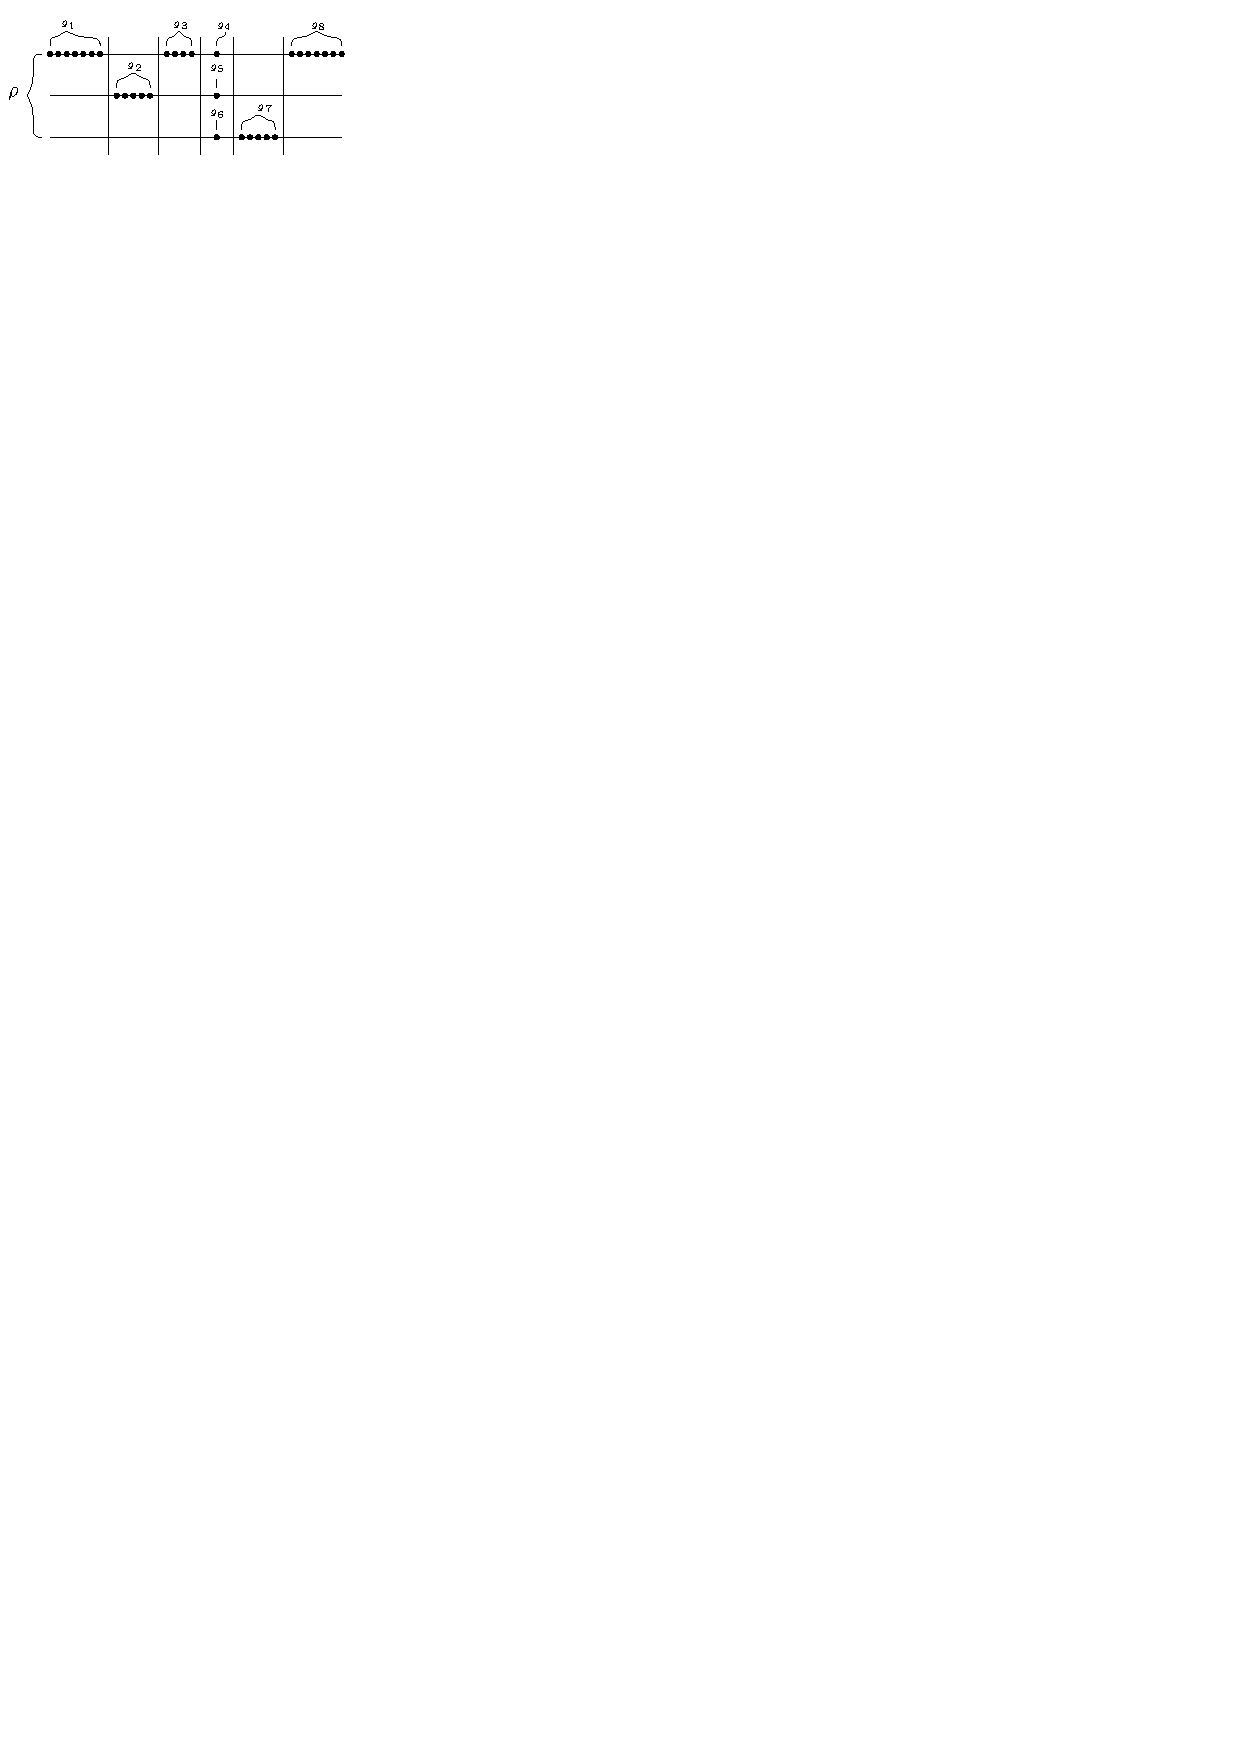
\includegraphics[scale=1.2]{union_instance1}
\end{minipage}\hfill
\begin{minipage}[c]{.45\textwidth}
  \captionof{figure}{An instance of the \textsc{Set Union} problem
    with $\rho=3$ sorted sets. In each set, the entry $\mathcal{A}[i]$ is
    represented by a point of $x$-coordinate $\mathcal{A}[i]$. The blocks
    that form the sets are noted. The blocks $g_4,g_5$ and $g_6$ are of
    size 1 because they correspond to elements of equal value and they
    induce the $4$-th member of the partition $\pi$ with value $m_4$
    equals $3$. The vertical bars separate the members of $\pi$.}
  \label{fig:instance}
\end{minipage}

We adapt the \texttt{DLM Union} algorithm for sorting a multiset.  The
algorithm \texttt{DLM Sort} detects the runs first through a linear
scan and then applies the algorithm \texttt{DLM Union}. After than,
transforming the output of the union algorithm to yield the sorted
multiset takes only linear time. The following corollary follows from
our refined analysis above:

\begin{corollary}
  Given a multiset $\mathcal{M}$ of size $n$ formed by $\rho$ runs and
  $\delta$ blocks of sizes $g_1, \dots, g_{\delta}$ such that these
  blocks induce a partition $\pi$ of size $\chi$ of the output whose
  members have values $m_1, \dots, m_{\chi}$, the algorithm {\tt{DLM Sort}} performs
  within
  $O(n + \sum^{\delta}_{i=1}\log g_i +
  \sum^{\chi}_{i=1}\log{\binom{\rho}{m_i}})$ data comparisons. This
  number of comparisons is optimal in the worst case over multisets of
  size $n$ formed by $\rho$ runs and $\delta$ blocks of sizes
  $g_1, \dots, g_{\delta}$ such that these blocks induce a partition
  $\pi$ of size $\chi$ of the output whose members have values
  $m_1, \dots, m_{\chi}$.
\end{corollary}

While the algorithm \texttt{DLM Sort} sorts multisets taking the best
advantage of both the \emph{input order} and the \emph{input
  structure} in a synergistic way, it does not yield a
\textsc{MultiSelection} algorithm nor a \textsc{Deferred Data
  Structure}. In the following section we
describe another sorting algorithm that also optimally takes advantage
of the local order and structure in the input, but which is based on a
distinct paradigm, more suitable to such extensions.

\subsubsection{Sorting Algorithm {\texttt{Quick Synergy
      Sort}}}
\label{sec:qss}

Given a multiset $\mathcal{M}$, the algorithm \texttt{Quick Synergy
  Sort} identifies the \emph{runs} in linear time through a scanning
process. \begin{LONG} As indicated by its name, the algorithm is
  directly inspired by the
  \texttt{QuickSort}~\cite{1961-CACM-Quicksort-Hoare}
  algorithm.\end{LONG} It computes a pivot $\mu$, which is the median
of the set formed by the middle elements of each run, and partitions
each \emph{run} by $\mu$. This partitioning process takes advantage of
the fact that the elements in each \emph{run} are already sorted. It
then recurses on the elements smaller than $\mu$ and on the elements
greater than $\mu$. (See Algorithm~\ref{alg:qss} for a more formal
description).

\begin{definition}[Median of the middles]
  Given a multiset $\mathcal{M}$ formed by runs, the ``\emph{median of
    the middles}'' is the median element of the set formed by the
  middle elements of each run.
\end{definition}

\begin{algorithm} % enter the algorithm environment
  \caption{\texttt{Quick Synergy Sort}} % give the algorithm a caption
  \label{alg:qss} % and a label for \ref{} commands later in the document
  \begin{algorithmic}[1] % enter the algorithmic environment

    \REQUIRE{A multiset $\mathcal{M}$ of size $n$} \ENSURE{A sorted sequence of
      $\mathcal{M}$}

    \STATE Compute the $\rho$ runs of respective sizes
    $(r_i)_{i\in[1..\rho]}$ in $\mathcal{M}$ such that
    $\sum^{\rho}_{i=1} r_i = n$;
    \STATE Compute the median $\mu$ of
    the middles of the runs, note $j\in[1..\rho]$ the run containing
    $\mu$;
    \STATE Perform doubling searches for the value $\mu$ in all
    runs except the $j$-th, starting at both ends of the runs in
    parallel;
    \STATE Find the maximum $\max_\ell$ (minimum $\min_r$)
    among the elements smaller (resp., greater) than $\mu$ in all runs
    except the $j$-th;
    \STATE Perform doubling searches for the values
    $\max_\ell$ and $\min_r$ in the $j$-th run, starting at the
    position of $\mu$;
    \STATE Recurse on the elements smaller than o
    equal to $\max_\ell$ and on the elements greater than or equal to
    $\min_r$.
  \end{algorithmic}
\end{algorithm}

The number of data comparisons performed by the algorithm
\texttt{Quick Synergy Sort} is asymptotically the same as the number
of data comparisons performed by the algorithm \texttt{DLM Sort}
described in the previous section.

\begin{theorem}
  Let $\mathcal{M}$ be a multiset of size $n$ formed by $\rho$ runs
  and $\delta$ blocks of sizes $g_1, \dots, g_{\delta}$ such that
  these blocks induce a partition $\pi$ of the output of size $\chi$
  whose members have values $m_1, \dots, m_{\chi}$. The algorithm
  \texttt{Quick Synergy Sort} performs within
  $O(n + \sum^{\delta}_{i=1} \log g_i +
  \sum^{\chi}_{i=1}\log{\binom{\rho}{m_i}})$ data comparisons on
  $\mathcal{M}$. This number of comparisons is optimal in the worst
  case over multisets of size $n$ formed by $\rho$ runs and $\delta$
  blocks of sizes $g_1, \dots, g_{\delta}$ such that these blocks
  induce a partition $\pi$ of size $\chi$ of the output whose members
  have values $m_1, \dots, m_{\chi}$.
\end{theorem}

Next, we generalize the algorithm \texttt{Quick Synergy Sort} to an
offline multiselection algorithm that partially sorts a multiset according to the set
of \texttt{select} queries given as input.

\subsection{MultiSelection Algorithm}
\label{sec:multiselect}

Given a linearly ordered multiset $\mathcal{M}$ and a sequence of
ranks $r_1, \dots, r_q$, a multiselection algorithm must answer the
queries \texttt{select}($r_1$), $\dots$, \texttt{select}($r_q$) in
$\mathcal{M}$, hence partially sorting $\mathcal{M}$.

Given a multiset $\mathcal{M}$ and a set of $q$ \texttt{select}
queries, the algorithm \texttt{Quick Synergy MultiSelection}
follows the same first steps as the algorithm \texttt{Quick Synergy
  Sort}. But once it has computed the ranks of all elements in the block that
contains the pivot $\mu$, it determines which \texttt{select} queries
correspond to elements smaller than or equal to $\max_\ell$ and which
ones correspond to elements greater than or equal to $\min_r$ (see
Algorithm~\ref{alg:qss} for the definitions of $\max_\ell$ and
$\min_r$). It then recurses on both sides.

We extend the notion of blocks to the context of partial sorting.

\begin{definition}[Pivot Blocks]
  Given a multiset $\mathcal{M}$ formed by $\rho$ runs and $\delta$
  blocks. The ``\emph{pivot blocks}'' are the blocks of $\mathcal{M}$
  that contain the pivots and the elements of value equals to the
  pivots during the steps of the algorithm \texttt{Quick Synergy
    MultiSelection}.
\end{definition}

In each run, between the pivot blocks and the insertion ranks of the
pivots, there are consecutive blocks that the algorithm \texttt{Quick Synergy
  MultiSelection} has not identified as separated blocks, because
no doubling searches occurred inside them.
 
\begin{definition}[Selection Blocks]
  Given the $i$-th run, formed of various blocks, and $q$
  \texttt{select} queries, the algorithm \texttt{Quick Synergy
    MultiSelection} computes $\xi$ pivots in the process of
  answering the $q$ queries. During the doubling searches,
  the algorithm \texttt{Quick Synergy MultiSelection} finds the insertion ranks
  of the $\xi$ pivots inside the $i$-th run. These positions determine
  a partition of size $\xi+1$ of the $i$-th run where each element of
  the partition is formed by consecutive blocks or is empty. We call
  the elements of this partition ``\emph{selection blocks}''. The
  set of all selection blocks include the set of all pivot blocks.
\end{definition}

Using these definitions, we generalize the results in Section~\ref{sec:syn-sort} to the more general problem of \textsc{MultiSelection}.

\begin{theorem}\label{theo:qsms}
  Given a multiset $\mathcal{M}$ of size $n$ formed by $\rho$ runs and
  $\delta$ blocks; and $q$ offline \texttt{select} queries over
  $\mathcal{M}$ corresponding to elements of \texttt{ranks}
  $r_1, \dots, r_q$. The algorithm \texttt{Quick Synergy
    MultiSelection} computes $\xi$ pivots in the process of answering
  the $q$ queries. Let $s_1,\dots, s_{\beta}$ be the sizes of the
  $\beta$ selection blocks determined by these $\xi$ pivots in all
  runs. Let $m_1, \dots, m_\lambda$ be the numbers of pivot blocks
  corresponding to the values of the $\lambda$ pivots with
  multiplicity greater than 1, respectively.  Let
  $\rho_0, \dots, \rho_\xi$ be the sequence where $\rho_i$ is the
  number of runs that have elements with values between the pivots $i$
  and $i+1$ sorted by \texttt{ranks}, for $i\in[1..\xi]$.  The
  algorithm \texttt{Quick Synergy MultiSelection} answers the $q$
  \texttt{select} queries performing within
  $O(n + \sum^{\beta}_{i=1}\log{s_i} +
    \beta\log{\rho}-\sum^{\lambda}_{i=1}m_i\log{m_i} -
    \sum^{\xi}_{i=0}\rho_i\log{\rho_i}) \subseteq
  O(n\log{n} - \sum^{q}_{i=0}\Delta_i\log{\Delta_i})$ data
  comparisons, where $\Delta_i = r_{i+1} - r_i$, $r_0=0$ and
  $r_{q+1}=n$.
\end{theorem}

In the result above, the queries are given all at the same time (i.e.,
offline). In the context where they arrive one at the time (i.e., online), we define
two \textsc{Deferred Data Structures} for answering online
\texttt{rank} and \texttt{select} queries, both inspired by the algorithm
\texttt{Quick Synergy MultiSelection}.

\subsection{Deferred Data Structures for MultiSets}
\label{sec:dds}

We describe two \textsc{Deferred Data Structures} that answer a set of \texttt{rank} and \texttt{select} queries arriving one at the time over a multiset $\mathcal{M}$, progressively sorting $\mathcal{M}$.  
%
Both data structures take advantage of the order (local and global) and structure in the input, and of the structure in the queries.
%
The first data structure is in the RAM model of computation, at the cost of not taking advantage of the order in which the queries are given. The second data structure is in the comparison model (a more constrained model) but does take advantage of the query order.

\subsubsection{Taking Advantage of  Order and Structure in the Input, but only of Structure in the Queries}

Given a multiset $\mathcal{M}$ of size $n$, the \textsc{RAM Deferred
  Data Structure} is composed of a bitvector $\mathcal{A}$ of size
$n$, in which we mark the elements in $\mathcal{M}$ that have been
computed as pivots by the algorithm when it answers the online
queries; a dynamic predecessor and successor structure $\mathcal{B}$
over the bitvector $\mathcal{A}$, which allows us to find the two
successive pivots between which the query fits; and for each pivot $p$
found, the data structure stores pointers to the insertion ranks of
$p$ in each run, to the beginning and end of the block $g$ to which
$p$ belongs, and to the position of $p$ inside $g$. The dynamic
predecessor and successor structure $\mathcal{B}$ requires the RAM
model of computation in order to answer \emph{predecessor and
  successor queries} in time within
$o(\log{n})$~\cite{2002-JCSS-OptimalBoundsForThePredecessorProblemAndRelatedProblems-BeameFich}.

\begin{theorem}\label{theo:online-ram}
  Consider a multiset $\mathcal{M}$ of size $n$ formed by $\rho$ runs and
  $\delta$ blocks. The \textsc{RAM Deferred Data Structure} computes
  $\xi$ pivots in the process of answering $q$ online \texttt{rank}
  and \texttt{select} queries over $\mathcal{M}$. Let
  $s_1, \dots, s_{\beta}$ be the sizes of the $\beta$ selection
  blocks determined by these $\xi$ pivots in all runs. Let
  $m_1, \dots, m_\lambda$ be the numbers of pivot blocks
  \begin{LONG}
    among this selection blocks
  \end{LONG}
  corresponding to the values of the $\lambda$ pivots with
  multiplicity greater than 1, respectively.  Let
  $\rho_0, \dots, \rho_\xi$ be the sequence where $\rho_i$ is the
  number of runs that have elements with values between the pivots $i$
  and $i+1$ sorted by \texttt{ranks}, for $i\in[1..\xi]$.  Let $u$ and
  $g_1, \dots, g_u $ be the number of \texttt{rank} queries and the
  sizes of the identified and searched blocks in the process of
  answering the $u$ \texttt{rank} queries, respectively. The
  \textsc{RAM Deferred Data Structure} answers these $q$ online
  \texttt{rank} and \texttt{select} queries in time within
  $O(n + \sum^{\beta}_{i=1}\log{s_i} + \beta\log{\rho} -
  \sum^{\lambda}_{i=1}m_i\log{m_i}
  - \sum^{\xi}_{i=0}\rho_i\log{\rho_i} + \xi\log\log{n} +
  u\log{n}\log\log{n} + \sum^{u}_{i=1}\log{g_i})$.
\end{theorem}

The \textsc{RAM Deferred Data Structure} takes advantage of the
structure in the queries and of the structure and order (local and
global) in the input. Changing the order in the \texttt{rank} and
\texttt{select} queries does not affect the time complexity of the
\textsc{RAM Deferred Data Structure}. Once the structure
  identifies the nearest pivots to the left and right of the query
  positions, the steps of the algorithms are the same as in the
  offline case (Section~\ref{sec:multiselect}). We
next describe a deferred data structure taking advantage of the
structure and order in the queries and of the structure and order
(local and global) in the input data.

\subsubsection{Taking Advantage of the Order and Structure in both the Input and the Queries}

To take advantage of the order in the queries, we introduce a
data structure that finds the nearest pivots to the left and to the
right of a position $p\in[1..n]$, while taking advantage of the
distance between the position of the last computed pivot and $p$. This
distance is measured in the number of computed pivots between the two
positions. For that we use a \emph{finger search
  tree}~\cite{1998-SODA-FingerSearchTreesWithConstantInsertionTime-Brodal}
which is a search tree maintaining \emph{fingers} (i.e., pointers) to
elements in the search tree. Finger search trees support efficient
updates and searches in the vicinity of the
fingers. Brodal~\cite{1998-SODA-FingerSearchTreesWithConstantInsertionTime-Brodal}
described an implementation of finger search trees that
searches for an element $x$, starting the search at the element given by
the finger $f$ in time within $O(\log{d})$, where $d$ is the distance
between $x$ and $f$ in the set (i.e, the difference between
\texttt{rank}$(x)$ and \texttt{rank}$(f)$ in the set). This operation
returns a finger to $x$ if $x$ is contained in the set, otherwise a
finger to the largest element smaller than $x$ in the set. This
implementation supports the insertion of an element $x$ immediately to
the left or to the right of a finger in \begin{LONG}worst-case\end{LONG} constant
time.

In the description of the \textsc{RAM Deferred Data Structure} from
Theorem~\ref{theo:online-ram}, we substitute the dynamic predecessor
and successor structure $\mathcal{B}$ by a finger search tree
$\mathcal{F}_{\texttt{select}}$, as described by
Brodal~\cite{1998-SODA-FingerSearchTreesWithConstantInsertionTime-Brodal}. Once
a block $g$ is identified, every element in $g$ is a valid pivot for
the rest of the elements in $\mathcal{M}$. In order to capture this
idea, we modify the structure $\mathcal{F}_{\texttt{select}}$ so that
it contains blocks (i.e., a sequence of consecutive values) instead of
singleton pivots. Each element in $\mathcal{F}_{\texttt{select}}$
points in $\mathcal{M}$ to the beginning and the end of the block $g$
that it represents and in each run to the position where the elements
of $g$ partition the run. This modification allows the structure to
answer \texttt{select} queries, taking advantage of the structure and
order in the queries and of the structure and order of the input
data. But in order to answer \texttt{rank} queries taking advantage of
the features in the queries and the input data, the structure needs
another finger search tree $\mathcal{F}_{\texttt{rank}}$. In
$\mathcal{F}_{\texttt{rank}}$ the structure stores for each block $g$
identified, the value of one of the elements in $g$, and pointers in
$\mathcal{M}$ to the beginning and the end of $g$ and in each run to
the position where the elements of $g$ partition the run. We name this
structure \textsc{Full-Synergistic Deferred Data Structure}.

\begin{theorem}\label{theo:finger}
  Consider a multiset $\mathcal{M}$ of size $n$ formed by $\rho$ runs and
  $\delta$ blocks. The \textsc{Full-Synergistic Deferred Data
    Structure} identifies $\gamma$ blocks in the process of answering
  $q$ online \texttt{rank} and \texttt{select} queries over
  $\mathcal{M}$ corresponding to elements of \texttt{ranks} $r_1,
  \dots, r_q$. Let $s_1, \dots, s_{\beta}$ be the sizes of the $\beta$
  selection blocks determined by the $\gamma$ blocks in all runs.
  Let
  $m_1, \dots, m_\lambda$ be the numbers of pivot blocks
  \begin{LONG}
    among this selection blocks
  \end{LONG}
  corresponding to the values of the $\lambda$ pivots with
  multiplicity greater than 1, respectively.  Let
  $\rho_0, \dots, \rho_\xi$ be the sequence where $\rho_i$ is the
  number of runs that have elements with values between the pivots $i$
  and $i+1$ sorted by \texttt{ranks}, for $i\in[1..\xi]$.  Let
  $d_1, \dots, d_{q-1}$ be the sequence where $d_j$ is the number
  of identified blocks between the block that answers the $j-1$-th
  query and the one that answers the $j$-th query before starting the
  steps to answer the $j$-th query, for $j\in[2..q]$. Let $u$ and
  $g_1, \dots, g_u $ be the number of \texttt{rank} queries and the
  sizes of the identified and searched blocks in the process of
  answering the $u$ \texttt{rank} queries, respectively. The
  \textsc{Full-Synergistic Deferred Data Structure} answers the $q$
  online
  \begin{LONG}
    \texttt{rank} and \texttt{select}
  \end{LONG}
queries performing within
  $O(n + \sum^{\beta}_{i=1}\log{s_i} + \beta\log{\rho} -
  \sum^{\lambda}_{i=1}m_i\log{m_i} -
  \sum^{\xi}_{i=0}\rho_i\log{\rho_i} + \sum^{q-1}_{i=1}\log{d_i} +
  \sum^{u}_{i=1}\log{g_i}) \subseteq O\left(n\log{n} -
    \sum^{q}_{i=0}\Delta_i\log{\Delta_i} + q\log{n}\right)$ data
  comparisons, where $\Delta_i = r_{i+1} - r_i$, $r_0=0$ and $r_{q+1}=n$.
\end{theorem}

Next, we describe three problems susceptibles to combinations of input
order and input structure techniques.

\section{Compressed Data Structures}
\label{sec:compressed}

Consider an array ${\mathcal{A}}[1..n]$ of $n$ comparable objects. A \emph{Range
  Minimum
  Query}~\cite{1993-SICOMP-RecursiveStarTreeParallelDataStructure-BerkmanVishkin}
consists of a pair of integers $i$ and $j$ such that
$1\le i\le j\le n$, and is answered by
\texttt{RMinQ}$_{\mathcal{A}}(i,j)$, the leftmost position of a
minimum in $\mathcal{A}[i..j]$. Such queries have a wide range of
applications in various data structures and algorithms, including text
indexing~\cite{2009-TCS-FasterEntropyBoundedCompressedSuffixTrees-FischerMakinenNavarro},
pattern
matching~\cite{2008-STACS-ImprovedAlgorithmsForTheRangeNextValueProblemAndApplications-CrochemoreIliopoulosKubicaRahmanWalen},
and more elaborate kinds of range
queries~\cite{2004-ISAAC-OnTheRangeMaximumSumSegmentQueryProblem-ChenChao}.

%%% RMQs in presence of Repetitions.

If the array $A$ is formed by repeated elements, then it is possible
to define more specific queries related to the
\texttt{RMinQ}$_{\mathcal{A}}(i,j)$ operation. The \emph{Range
  Leftmost Minimun Queries} (\texttt{RLMinQ}$_{\mathcal{A}}(i,j)$),
\emph{Range Rightmost Minimun Queries}
(\texttt{RRMinQ}$_{\mathcal{A}}(i)$) and \emph{Range k-th Minimum
  Query} (\texttt{RkMinQ}$_{\mathcal{A}}(i,j)$) return, given $m$
elements of minimum values of ranks $r_1, \dots, r_m$ in the range
${\mathcal{A}}[i..j]$, $r_1$, $r_m$ and $r_k$, respectively.
%%% PSVs Similar kind of queries are \emph{Previous Smaller Value}
\texttt{PSV}$_{\mathcal{A}}(i)$ and \emph{Previous Larger Value}
\texttt{PLV}$_{\mathcal{A}}(i)$, which return the position of the nearest
smaller/larger value among ${\mathcal{A}}[1..i]$, by analogy the operations
\emph{Next Smaller Value} \texttt{NSV}$_{\mathcal{A}}(i)$ and \emph{Next Larger Value}
\texttt{NLV}$_{\mathcal{A}}(i)$ can be defined.

Fischer~\cite{2010-LATIN-OptimalSuccinctnessForRangeMinimumQueries-Fischer}
described a non-systematic succinct index (which does not access the
original data when answering queries) using $2n+o(n)$ bits and
supporting RMQs in zero accesses to $\mathcal{A}$ and $O(1)$ accesses to the
index, which can be built in $O(n)$ time.

%%% Multiple Operations
Gawrychowski and
Nicholson~\cite{2015-ICALP-OptimalEncodingsForRangeTopKSelectionAndMinMax-GawrychowskiNicholson},
among other results, gave an index to support \emph{Range Minimum
  Query} and \emph{Range Maximum Query}
(\texttt{RMaxQ}$_{\mathcal{A}}(i,j)$) in constant time using
$3n + o(n)$ bits.
Fischer~\cite{2011-TCS-CombinedDataStructureForPreviousAndNextSmallerValues-Fischer}
described a non-systematic succinct index using $2.54n + o(n)$ to
support \texttt{PSV}$_{\mathcal{A}}(i)$,
\texttt{NSV}$_{\mathcal{A}}(i)$ and
\texttt{RMinQ}$_{\mathcal{A}}(i,j)$. By combining both approaches, Jo
and
Rao~\cite{2015-COCOON-SimultaneousEncodingsForRangeAndNextPreviousLargerSmallerValueQueries-JoRao}
described encodings that support a wide range of queries: an encodings
using $3.322n + o(n)$ bit that supports
\texttt{RMinQ}$_{\mathcal{A}}(i,j)$,
\texttt{RMaxQ}$_{\mathcal{A}}(i,j)$,
\texttt{RRMinQ}$_{\mathcal{A}}(i,j)$,
\texttt{RRMaxQ}$_{\mathcal{A}}(i,j)$, \texttt{PSV}$_{\mathcal{A}}(i)$
and \texttt{PLV}$_{\mathcal{A}}(i)$ in constant time and an encoding
using $4.585n + o(n)$ bits that supports
\texttt{RMinQ}$_{\mathcal{A}}(i,j)$,
\texttt{RRMinQ}$_{\mathcal{A}}(i,j)$,
\texttt{RLMinQ}$_{\mathcal{A}}(i,j)$,
\texttt{RkMinQ}$_{\mathcal{A}}(i,j)$, \texttt{PSV}$_{\mathcal{A}}(i)$,
\texttt{NSV}$_{\mathcal{A}}(i)$, \texttt{RMaxQ}$_{\mathcal{A}}(i,j)$,
\texttt{RRMaxQ}$_{\mathcal{A}}(i,j)$,
\texttt{RLMaxQ}$_{\mathcal{A}}(i,j)$,
\texttt{RkMaxQ}$_{\mathcal{A}}(i,j)$, \texttt{PLV}$_{\mathcal{A}}(i)$,
\texttt{NLV}$_{\mathcal{A}}(i)$ in constant time.

%%% Input Order Compression of RMQs
In the worst case over all
possible arrays of $n$ comparable objects, any fully separated index
requires at least $2n$ bits in order to support such queries.
% 
When the array ${\mathcal{A}}$ is composed of $\rho \in o(n)$ runs,
Barbay et
al.~\cite{2012-TCS-LRMTreesCompressedIndicesAdaptiveSortingAndCompressedPermutations-BarbayFischerNavarro}
described a systematic compressed index using
$\lg{n\choose \rho} + o(n)$ bits, that can be computed in
$n-1+2(\rho-1) \in n+o(n)$ data comparisons and $O(n)$ overall time,
and supports \texttt{RMinQ}$_{\mathcal{A}}(i,j)$ in $1$ comparison
within ${\mathcal{A}}$ and $O(1)$ accesses to the index. This
compressed data structure takes advantage of the order of the elements
in the input.

Taking advantage of the repetitions in multisets is unlikely to yield
much better results for \emph{Range Minimum Query} indexes given that,
from the point of view of \emph{Range Minimum Query} indexes,
instances varying in repetitions such as $(2,1,3)$ and $(2, 1, 2)$ are
indistinguishable.

\textbf{\begin{enumerate}
  \item Is there a compressed index for ${\mathcal{A}}$ that supports a wide range
of operations which takes advantage of the number and sizes of the
\emph{runs} that form ${\mathcal{A}}$?
  \item Is there a compressed index for ${\mathcal{A}}$ that supports a wide range
of operations which takes advantage of the repetitions in ${\mathcal{A}}$?
  \item Is there a compressed index for ${\mathcal{A}}$ that supports a wide range
of operations which takes advantage of the number and sizes of the
\emph{runs} and the repetitions in ${\mathcal{A}}$ in a synergistic way, so that
it takes less space on instances where it can take advantage of both
at the same time?
  \end{enumerate} }

\section{Maxima Solutions}
\label{sec:maxima}

\section{Convex Hull Solutions}
\label{sec:hull}

We improve the analysis of this algorithm including not only the
minimum number of simple subchain into which the polygonal chain can
be partitioned but also their sizes.


\section{Conclusion}
\label{sec:con}

We predict that such analysis techniques will take on more importance
in the future, along with the growth of the block between practical
cases and the worst case over instances of fixed sizes. Furthermore,
we conjecture that synergistic techniques taking advantage of more
than one ``easiness'' aspect will be of practical importance if the
block between theoretical analysis and practice is to ever be reduced.

%%% Local Variables:
%%% mode: latex
%%% TeX-master: "2016-ThesisProposal-Ochoa"
%%% End:
